
\documentclass{beamer}
\usecolortheme{dove}
\setbeamertemplate{navigation symbols}{}
\usepackage{amsmath,amssymb,amsfonts,amsthm, multicol, subfigure, color}
\usepackage{bm}
\usepackage{graphicx}
\usepackage{tabularx}
\usepackage{booktabs}
\usepackage{hyperref}
\usepackage{pdfpages}
\usepackage{xcolor}
\definecolor{seagreen}{RGB}{46, 139, 87}
\definecolor{mustard}{RGB}{234, 170, 0}
\def\independenT#1#2{\mathrel{\rlap{$#1#2$}\mkern2mu{#1#2}}}
\newcommand\indep{\protect\mathpalette{\protect\independenT}{\perp}}
\def\log{\text{log}}
\newcommand\logit{\text{logit}}
\newcommand\iid{\stackrel{\text{iid}}{\sim}}
\newcommand\E{\text{E}}
\newcommand\V{\text{V}}
\renewcommand\P{\text{P}}
\newcommand{\Cov}{\text{Cov}}
\newcommand{\Cor}{\text{Cor}}
\newcommand\doop{\texttt{do}}
\usepackage{stackrel}
\usepackage{tikz}
\usetikzlibrary{arrows,shapes.arrows,positioning,shapes,patterns,calc}
\newcommand\slideref[1]{\vskip .1cm \tiny \textcolor{gray}{{#1}}}
\newcommand\red[1]{\color{red}#1}
\newcommand\blue[1]{\color{blue}#1}
\newcommand\gray[1]{\color{gray}#1}
\newcommand\seagreen[1]{\color{seagreen}#1}
\newcommand\purple[1]{\color{purple}#1}
\newcommand\orange[1]{\color{orange}#1}
\newcommand\black[1]{\color{black}#1}
\newcommand\white[1]{\color{white}#1}
\newcommand\teal[1]{\color{teal}#1}
\newcommand\magenta[1]{\color{magenta}#1}
\newcommand\Fuchsia[1]{\color{Fuchsia}#1}
\newcommand\BlueGreen[1]{\color{BlueGreen}#1}
\newcommand\bblue[1]{\textcolor{blue}{\textbf{#1}}}
\newcommand\bred[1]{\textcolor{red}{\textbf{#1}}}
\newcommand\bgray[1]{\textcolor{gray}{\textbf{#1}}}
\newcommand\bgreen[1]{\textcolor{seagreen}{\textbf{#1}}}
\newcommand\bref[2]{\href{#1}{\color{blue}{#2}}}
\colorlet{lightgray}{gray!40}
\pgfdeclarelayer{bg}    % declare background layer for tikz
\pgfsetlayers{bg,main} % order layers for tikz
\newcommand\mycite[1]{\begin{scriptsize}\textcolor{darkgray}{(#1)}\end{scriptsize}}
\newcommand{\tcframe}{\frame{
%\small{
\only<1|handout:0>{\tableofcontents}
\only<2|handout:1>{\tableofcontents[currentsubsection]}}
%}
}

\newcommand{\goalsframe}{\begin{frame}{Learning goals for today}
By the end of class, you will be able to
\begin{itemize}
    \item define causal effects using potential outcomes
    \item understand the fundamental problem of causal inference
\end{itemize} \vskip .2in
\end{frame}}

\usepackage[round]{natbib}
\bibliographystyle{humannat-mod}
\setbeamertemplate{enumerate items}[default]
\usepackage{mathtools}

\title{Studying Social Inequality with Data Science}
\author{Ian Lundberg}
\date{\today}

\begin{document}

\begin{frame}
\begin{tikzpicture}[x = \textwidth, y = \textheight]
\node at (0,0) {};
\node at (1,1) {};
\node[anchor = north west, align = left, font = \huge] at (0,.9) {Studying\\Social Inequality\\with Data Science};
\node[anchor = north east, align = right] (number) at (1,.9) {INFO 3370 / 5371\\Spring 2023};
\node[anchor = north, font = \Large, align = left] at (.5,.5) {\bblue{Interventions to Promote Equality:}\\\bblue{Causal inference}};
\end{tikzpicture}
\end{frame}

\goalsframe

\begin{frame}{Class module: Interventions to promote equality}

\begin{itemize}
\item don't just study the world
\item learn how we might change it
\end{itemize}

\end{frame}

\begin{frame}{Education: A tool to promote opportunity}

\includegraphics[width = \textwidth]{figures/hout_educReturns}

\end{frame}

\begin{frame}{Two claims}


\begin{tikzpicture}[x = \textwidth, y = .8\textheight]
\node at (0,0) {};
\node at (1,1) {};
\node[anchor = north west, align = left] at (.05,1) {People with\\college degrees\\earn more};
\node[anchor = north west, align = left] at (.55,1) {A college degree\\causes\\higher earnings};
\node<2>[anchor = north west, font = \large, align = left] at (0.05,.7) {What policies would each claim support?};
\node<3-6>[anchor = north west, align = left] at (0.05,.7) {Two sets of people\\Two treatments};
\only<4->{
\draw[rounded corners, fill = blue, fill opacity = .3] (.05,.3) rectangle (.25,.5) {};
\draw[rounded corners, fill = seagreen, fill opacity = .3] (.25,.1) rectangle (.45,.3) {};
\node[anchor = north, align = center, font = \footnotesize, blue] at (.15, .1) {Outcome\\with college};
\node[anchor = north, align = center, font = \footnotesize, seagreen] at (.35, .1) {Outcome\\without};
\node[anchor = south, rotate = 90, align = center] at (.05, .3) {People};
}
\node<5-7>[anchor = north west, align = left] at (.55,.7) {Same people\\Two treatments};
\only<6->{
\draw[rounded corners, fill = blue, fill opacity = .3] (.55,.1) rectangle (.75,.5) {};
\draw[rounded corners, fill = seagreen, fill opacity = .3] (.75,.1) rectangle (.95,.5) {};
\node[anchor = north, align = center, font = \footnotesize, blue] at (.65, .1) {Outcome\\with college};
\node[anchor = north, align = center, font = \footnotesize, seagreen] at (.85, .1) {Outcome\\without};
\node[anchor = south, rotate = 90, align = center] at (.55, .3) {People};
}
\node<7-> at (.15, .4) {$Y_i$};
\node<7-> at (.35, .2) {$Y_i$};
\node<8-> at (.65, .3) {$Y_i^\text{College}$};
\node<8->[font = \small] at (.85, .3) {$Y_i^\text{Non-college}$};
\only<7->{
\node[anchor = north, align = center] (factual) at (.25,.7) {factual\\outcomes};
\draw[->, thick] (.2,.55) -- (.15,.45);
\draw[->, thick] (.3,.55) -- (.35,.25);
}
\only<8->{
\node[anchor = north, align = center] (potential) at (.75,.7) {potential\\outcomes};
\draw[->, thick] (.7,.55) -- (.65,.35);
\draw[->, thick] (.8,.55) -- (.85,.35);
}
\node<9->[anchor = north east, align = right, font = \footnotesize, gray] at (1,.7) {\href{https://catalog.library.cornell.edu/catalog/12108069}{Imbens \&}\\\href{https://catalog.library.cornell.edu/catalog/12108069}{Rubin}\\\href{https://catalog.library.cornell.edu/catalog/12108069}{2015}};
\end{tikzpicture}

\end{frame}

\begin{frame}{Translate causal statements to potential outcomes}

\begin{tikzpicture}[x = \textwidth, y = .9\textheight]
\node at (0,0) {};
\node at (1,1) {};
\node<8->[anchor = north] at (.5,.9) {\bblue{Is it possible to know if each statement is true?}};
\only<2->{
\node[anchor = north west, align = left] at (0,.8) {1)};
\node[anchor = north west, align = left] at (0.05,.8) {
Sarah would have been hired\\
if she had submitted her\\
application on time
};
}
\only<3->{
\node[anchor = north east, align = right] at (1,.8) {$\begin{aligned}&Y_\text{Sarah}^\text{On time} &= 1\\&Y^\text{Late}_\text{Sarah} &= 0\end{aligned}$};
}
\only<4->{
\node[anchor = north west, align = left] at (0,.6) {2)};
\node[anchor = north west, align = left] at (0.05,.6) {
David would have been\\hired even if he hadn't\\had a college degree
};
\node[anchor = north west, align = left] at (0,.4) {3)};
\node[anchor = north west, align = left] at (0.05,.4) {
The hiring manager discriminatorily\\chose Emily over Lakisha\\because of their names
};
\node[anchor = north west, align = left] at (0,.2) {4)};
\node[anchor = north west, align = left] at (0.05,.2) {
Juan never even applied because\\
he has a newborn infant
};
}
\node<5->[anchor = north east, align = right] at (1,.6) {$\begin{aligned} &Y_\text{David}^\text{College} &= 1\\&Y_\text{David}^\text{Non-college} &= 1\end{aligned}$};
\node<6->[anchor = north east, align = right] at (1,.4) {$\begin{aligned}&Y_\text{Lakisha}^\text{Named Emily} &= 1\\&Y_\text{Lakisha}^\text{Named Lakisha} &= 0\end{aligned}$};
\node<7->[anchor = north east, align = right] at (1,.2) {$\begin{aligned}&Y_\text{Juan}^\text{Infant} &= 0\\&Y_\text{Juan}^\text{No infant} &= 1\end{aligned}$};
\end{tikzpicture}

\end{frame}

\begin{frame}{\onslide<5->{Average causal effects}}
\begin{tikzpicture}[x = \textwidth, y = .8\textheight]
\node at (0,0) {};
\node at (1,1) {};
\node<2-4>[anchor = north west, align = left] at (0,1) {Could we ever know the effect for person 1?\\\only<3-4>{For anyone?}\\\only<4>{Can anything be known?}};
\node<2-4>[anchor = south east, gray, font = \bf] at (1,0) {\href{https://www.tandfonline.com/doi/abs/10.1080/01621459.1986.10478354}{Holland 1986}};
\node<6->[anchor = north, align = center, font = \small] at (.5,1) {If treatment is randomized,\\then the observed cases\\in each treatment condition\\are a simple random sample};
% Individual outcomes
\node[anchor = north west, font = \bf] at (.05,.7) {The data};
\foreach \i in {.2,.3,.35,.45,.55} {
	\draw[fill = blue, opacity = .3, color = blue] (.05,\i) rectangle (.25,\i + .05) {};
}
\foreach \i in {.25,.4,.5} {
	\draw[fill = seagreen, opacity = .3, color = seagreen] (.25,\i) rectangle (.45,\i + .05) {};
}
\node[font = \tiny] at (.15,.575) {$Y_1^1$};
\node[font = \tiny] at (.35,.525) {$Y_2^0$};
\node[font = \tiny] at (.15,.475) {$Y_3^1$};
\node[font = \tiny] at (.35,.425) {$Y_4^0$};
\node[font = \tiny] at (.15,.375) {$Y_5^1$};
\node[font = \tiny] at (.15,.325) {$Y_6^1$};
\node[font = \tiny] at (.35,.275) {$Y_7^0$};
\node[font = \tiny] at (.15,.225) {$Y_8^1$};
\node[anchor = north, align = center, font = \footnotesize, blue] at (.15, .2) {Outcome\\under\\treatment};
\node[anchor = north, align = center, font = \footnotesize, seagreen] at (.35, .2) {Outcome\\under\\control};
\node[anchor = south, rotate = 90, align = center] at (.05, .4) {People};
% Average outcomes
\onslide<5->{
\node[anchor = north west, font = \bf] at (.55,.7) {The claim};
\draw[fill = blue, color = blue, opacity = .3] (.55,.2) rectangle (.75,.6) {};
\draw[fill = seagreen, color = seagreen, opacity = .3] (.75,.2) rectangle (.95,.6) {};
\node[anchor = north, align = center, font = \footnotesize, blue] at (.65, .2) {Outcome\\under\\treatment};
\node[anchor = north, align = center, font = \footnotesize, seagreen] at (.85, .2) {Outcome\\under\\control};
\node[anchor = south, rotate = 90, align = center] at (.55, .4) {People};
\node[align = center] at (.65,.4) {Average\\$\bar{Y}^1$};
\node[align = center] at (.85,.4) {Average\\$\bar{Y}^0$};
}
\end{tikzpicture}
\end{frame}

\goalsframe

\begin{frame}
\huge Bonus slides
\end{frame}

\begin{frame}

For each statement, draw a table of potential outcomes.
\begin{itemize}
\item Who are the people being considered?
\item Under what treatment conditions?
\item What potential outcome is obseverved?
\end{itemize} \vskip .1in
Statements
\begin{enumerate}
\item On average, those who attend college have higher annual earnings than what they would have earned without college
\item On average, those who did not attend college would earn more if they attended college
\item On average, the causal effect of college on earnings is higher for those whose parents did not attend college
\end{enumerate}
\end{frame}

\begin{frame}
Challenge: \vskip .2in
Visitors to the Cornell Dairy Bar would be more impressed if they ordered Cascadilla Cookies \& Cream than if they ordered French Vanilla, but they would be most impressed if they ordered Big Red Bear Tracks.
\end{frame}



\end{document}

